\documentclass[conference,a4paper]{IEEEtran}
\IEEEoverridecommandlockouts

\usepackage[T1]{fontenc}
\usepackage{cite}
\usepackage{amsmath,amssymb,amsfonts,mathtools}
\usepackage{algorithmic}
\usepackage{graphicx}
\usepackage{textcomp}
\usepackage{xcolor}
\usepackage{flushend}
\usepackage{fancyhdr}
\usepackage{balance}
\usepackage{multirow}
\usepackage{array}
\usepackage{tabu}
\usepackage{color}
\usepackage{ragged2e}
\usepackage{microtype}
\usepackage{url}
\def\UrlBreaks{\do\/\do-\do\_}

\def\BibTeX{{\rm B\kern-.05em{\sc i\kern-.025em b}\kern-.08em
    T\kern-.1667em\lower.7ex\hbox{E}\kern-.125emX}}
 
\renewcommand\IEEEkeywordsname{Keywords}

\setlength{\headheight}{13mm}
% Page Layout setup
\voffset = 4mm
\headsep = 16pt
\textwidth = 182mm
\textheight = 238mm
\footskip = 12.157mm
\usepackage{hyperref}
\usepackage{listings}

\usepackage{pgfplots}
\usepackage{pgfplotstable}
\pgfplotsset{compat=1.18}

% Define colors for syntax highlighting

\definecolor{codegreen}{rgb}{0,0.6,0}
\definecolor{codegray}{rgb}{0.5,0.5,0.5}
\definecolor{codepurple}{rgb}{0.58,0,0.82}
\definecolor{backcolour}{rgb}{0.95,0.95,0.92}

\lstdefinestyle{mystyle}{
    backgroundcolor=\color{backcolour},   
    commentstyle=\color{codegreen},
    keywordstyle=\color{magenta},
    numberstyle=\tiny\color{codegray},
    stringstyle=\color{codepurple},
    basicstyle=\ttfamily\scriptsize,
    breakatwhitespace=false,         
    breaklines=true,                 
    captionpos=b,                    
    keepspaces=true,                 
    numbers=left,                    
    numbersep=5pt,                  
    showspaces=false,                
    showstringspaces=false,
    showtabs=false,                  
    tabsize=2,
    columns=fullflexible
}

% C++ language definition
\lstdefinelanguage{ModernC++}{
  keywords={alignas, alignof, and, and_eq, asm, atomic_cancel, atomic_commit, atomic_noexcept, auto, bitand, bitor, bool, break, case, catch, char, char8_t, char16_t, char32_t, class, compl, concept, const, consteval, 
  constexpr, constinit, const_cast, continue, contract_assert, co_await, co_return, co_yield, decltype, default, delete, do, double, dynamic_cast, else, enum, explicit, export, extern, false, float, for, friend, goto, if, inline, int, long, mutable, namespace, new, noexcept, not, not_eq, nullptr, operator, or, or_eq, private, protected, public, reflexpr, register, reinterpret_cast, requires, return, short, signed, sizeof, static, static_assert, static_cast, struct, switch, synchronized, template, this, thread_local, throw, true, try, typedef, typeid, typename, union, unsigned, using, virtual, void, volatile, wchar_t, while, xor, xor_eq},
  sensitive=true,
  morecomment=[l]//,
  morestring=[b]',
  morestring=[b]",
  showstringspaces=false,
  basicstyle=\ttfamily\scriptsize              
}

% Python language definition
\lstdefinelanguage{Python}{
  morekeywords={
    def, return, if, elif, else, while, for, in, try, except, finally, 
    class, from, import, as, pass, raise, break, continue, lambda, 
    with, assert, yield, del, global, nonlocal, True, False, None
  },
  sensitive=true,
  morecomment=[l]\#,
  morestring=[b]',
  morestring=[b]",
  showstringspaces=false,
  basicstyle=\ttfamily\small
}

% JavaScript language definition
\lstdefinelanguage{JavaScript}{
  keywords={typeof, new, true, false, catch, function, return, null, catch, switch, var, if, in, while, do, else, case, break, const, let,
  class, export, boolean, throw, implements, import, this, constructor},
  sensitive=true,
  morecomment=[l]//,
  morestring=[b]',
  morestring=[b]",
  showstringspaces=false,
  basicstyle=\ttfamily\small
}

\lstset{style=mystyle}

\begin{document}

\newcounter{tblEqCounter} %create a counter

\title{{\fontsize{21}{14.4}\selectfont
Zero-Codegen Protocol Buffers via C++26 Static Reflection and Compile-Time Metaprogramming}%
\thanks{\textsuperscript{1}Alex I. Tsvetanov is with the Faculty of Computer Systems and Technologies, Technical University of Sofia, ul. Professor Georgi Bradistilov 11, Sofia, Bulgaria (E-mail: \href{mailto:atsvetanov@tu-sofia.bg}{atsvetanov@tu-sofia.bg}).}%
}

\author{
\IEEEauthorblockN{{\fontsize{14}{14.4}\selectfont
Alex I. Tsvetanov\textsuperscript{1}}}
}

\maketitle

\pagenumbering{arabic}
\setcounter{page}{1}
\renewcommand{\headrulewidth}{0pt}
\renewcommand{\footrulewidth}{0pt}
\thispagestyle{fancy}
	\chead{{\fontsize{10}{13.0}\selectfont
International Scientific Conference on Computer Science and Information Technologies, 2026}  }
    \fancyfoot[C]{\thepage}

\begin{abstract}
Protocol Buffers rely on an external code generator, \texttt{protoc}, which a build must
invoke to produce intermediate C++ files, and which brings custom build rules, version skew
between the generator and the runtime library, and hundreds of thousands of generated lines
in a large system. This paper presents \texttt{ctpb}, a header-only C++26 library that removes
the generator by moving schema ingestion into the compiler front end, uniting P1967
\texttt{\#embed} with P2996 static reflection so that a three-stage \texttt{constexpr}
pipeline tokenizes a \texttt{.proto} schema, parses it to an abstract syntax tree during
constant evaluation, and materializes it as first-class C++ structs with wire visitors. Two
different costs are reported and should not be confused: the parser itself, compiled at
\texttt{-O3} and executed at run time, processes the largest schema tested in under
$11.4\,\mu\text{s}$, whereas the cost a build actually pays is incurred inside constant
evaluation, and is bounded there not by memory but by the compiler's step limit, a single
message of 300 \texttt{int32} fields compiling under Clang's default of $1{,}048{,}576$ steps
and one of 301 not. At run time the generated code encodes at $1{,}396.0\,\text{MiB/s}$ and
decodes at $350.2\,\text{MiB/s}$, $2.81\times$ and $1.71\times$ over Google's
\texttt{libprotobuf} and holding against the leaner \texttt{libprotobuf-lite}, with
bidirectional wire-format fidelity verified against the reference implementation and a
stripped static executable of $18.3\,\text{KB}$ against $1.72\,\text{MB}$. Two limits bound
the claim: P2996 exists only in experimental compiler branches pending ISO C++26
ratification, so this is a demonstration of feasibility rather than a deployable library, and
unknown fields are skipped rather than preserved, which differs in semantics from the
reference implementation for any endpoint that re-encodes what it received.
\end{abstract}

\begin{IEEEkeywords}
Protocol Buffers, C++26, Static Reflection, \#embed, Compile-Time Metaprogramming, Zero-Codegen Serialization
\end{IEEEkeywords}

\section{Introduction}

Interface Definition Languages (IDLs) such as Google Protocol Buffers (Protobuf) \cite{protobuf_spec}, FlatBuffers \cite{flatbuffers}, and Cap'n Proto \cite{capnproto} have become foundational to distributed systems, microservice architectures, and high-performance computing. Protocol Buffers provide cross-language interoperability, compact wire encodings, and robust backward- and forward-compatibility guarantees.

Historically, Protocol Buffers rely on an external code generator, \texttt{protoc}. When compiling a C++ project that utilizes Protobuf schemas, the build system must execute \texttt{protoc} to generate intermediate \texttt{.pb.h} header files and \texttt{.pb.cc} implementation files. While functional, this workflow introduces substantial engineering friction:

\begin{itemize}
    \item \textbf{Build System Complexity:} Incorporating external code generators requires intricate build rules (such as CMake \texttt{add\_custom\_command} or Bazel rules), tracking dependency directed acyclic graphs (DAGs), and synchronizing generator toolchains across development and production environments.
    \item \textbf{Version Skew and Toolchain Synchronization:} Mismatches between the runtime \texttt{libprotobuf} library and the build-time \texttt{protoc} compiler binary frequently produce subtle ABI incompatibilities or compilation failures.
    \item \textbf{Codebase Bloat and Intermediate Artifacts:} For large enterprise systems with hundreds of messages, generated header files span hundreds of thousands of lines of code, placing significant memory pressure on compiler front-ends and slowing incremental builds.
    \item \textbf{Loss of Direct Language Integration:} Developers must maintain external build targets rather than expressing message schemas as native, compile-time entities within the C++ type system.
\end{itemize}

With the upcoming ISO C++26 standard, the language introduces two transformative features: P1967 \texttt{\#embed} \cite{p1967} for zero-overhead compile-time file inclusion, and P2996 Static Reflection \cite{p2996} with splicing operators for programmatic type synthesis. 

In this paper, we present \texttt{ctpb} (Compile-Time Protobuf) \cite{ctpb2026}, a header-only modern C++26 library that eliminates the external \texttt{protoc} code generator entirely. \texttt{ctpb} embeds \texttt{.proto} schema files directly into the translation unit at compile time, executes a fully \texttt{constexpr} recursive-descent parser inside the compiler front-end, and synthesizes type-safe C++ structs, accessors, and wire-format serialization routines through static reflection.

The primary contributions of this work are:
\begin{enumerate}
    \item We design a three-stage compile-time architecture that transforms raw IDL text into first-class C++ types entirely within the compiler front-end without intermediate disk I/O.
    \item We implement a zero-allocation, \texttt{constexpr} recursive-descent proto3 parser capable of validating schemas, parsing nested messages, enums, maps, oneofs, and reserved ranges at compile time.
    \item We demonstrate the application of C++26 P2996 static reflection to programmatically inject member fields, wire visitors, and equality operators.
    \item We evaluate \texttt{ctpb}'s compile-time and runtime performance, showing schema parsing latencies under $11.4\,\mu\text{s}$ and wire serialization throughput exceeding $300\,\text{MB/s}$.
\end{enumerate}

\section{Background and Motivation}

\subsection{Protocol Buffers Specification}
Protocol Buffers define a compact, extensible binary wire format based on field tags and wire types. Each field transmitted across the wire begins with a key represented as a variable-length integer (varint) computed as:
\begin{equation}
\text{Key} = (\text{Field Number} \ll 3) \mid \text{Wire Type}
\label{eq:wire_key}
\end{equation}

The proto3 specification standardizes six wire types (Table~\ref{tab:wire_types}), with types 3 and 4 deprecated in modern protocols.

\begin{table}[ht]
\centering
\caption{Protocol Buffers Wire Type Mapping}
\label{tab:wire_types}
\renewcommand{\arraystretch}{1.15}
\setlength{\tabcolsep}{2.5pt}
\scriptsize
\begin{tabular}{|c|l|p{4.2cm}|}
\hline
\textbf{ID} & \textbf{Wire Format} & \textbf{Associated Scalar Types} \\ \hline
0 & Varint & \raggedright \texttt{int32, int64, uint32, uint64, bool, enum} \tabularnewline \hline
1 & 64-bit Fixed & \texttt{fixed64, sfixed64, double} \\ \hline
2 & Length-delim. & \texttt{string, bytes}, submessages, packed \\ \hline
5 & 32-bit Fixed & \texttt{fixed32, sfixed32, float} \\ \hline
\end{tabular}
\end{table}

Signed integers (\texttt{sint32}, \texttt{sint64}) use Zigzag encoding to map signed quantities to unsigned integers with minimal high-order bits:
\begin{align}
\text{Zigzag}_{32}(n) &= (n \ll 1) \oplus (n \gg 31) \\
\text{Zigzag}_{64}(n) &= (n \ll 1) \oplus (n \gg 63)
\end{align}

\subsection{P1967: Resource Inclusion via \#embed}
Before C++26, embedding non-C++ assets (such as IDL files, shaders, or schemas) into a translation unit required external build scripts generating C-style byte arrays (e.g., via \texttt{xxd -i}) or string literals. Proposal P1967 \cite{p1967} adds the \texttt{\#embed} preprocessor directive:
\begin{lstlisting}[language=ModernC++]
constexpr char proto_source[] = {
    #embed "addressbook.proto"
};
\end{lstlisting}
The compiler exposes the embedded binary content as a contiguous memory span directly inside the compiler front-end with zero runtime copying or separate build steps.

\subsection{P2996: Static Reflection in C++26}
Proposal P2996 \cite{p2996} provides a comprehensive static reflection facility for C++26 centered around the \texttt{std::meta::info} opaque type and the splice operator \texttt{[: ... :]}. Static reflection operates in three key dimensions:
\begin{itemize}
    \item \textbf{Introspection:} Querying entity properties and metadata (e.g., \texttt{\^{}\^{}T}, \texttt{members\_of()}).
    \item \textbf{Generation:} Programmatically synthesizing member descriptors via builders (\texttt{define\_aggregate()}, \texttt{data\_member\_spec()}).
    \item \textbf{Splicing:} Materializing reflected meta-entities into concrete declarations using \texttt{[: r :]}.
\end{itemize}

Combined with \texttt{constexpr} evaluation, P2996 turns the C++ compiler into a programmable meta-compiler capable of digesting external domain-specific languages and generating optimal native types.

\section{Architecture and Compile-Time Pipeline}

The core architecture of \texttt{ctpb} is organized as a three-stage compile-time compilation pipeline executing entirely within the host compiler front-end prior to code emission (Fig.~\ref{fig:ctpb_pipeline}).

\begin{figure*}[ht]
\centering
\begin{tikzpicture}[
    box/.style={
        rectangle, 
        draw=black!75, 
        thick, 
        minimum width=3.1cm, 
        minimum height=1.3cm, 
        align=center, 
        rounded corners=4pt, 
        font=\footnotesize
    },
    arrow/.style={
        ->, 
        >=stealth, 
        line width=1.1pt, 
        draw=black!75
    },
    labelnode/.style={
        midway, 
        above=4pt, 
        font=\scriptsize\sffamily, 
        text=black!85
    }
]
\node[box, fill=orange!15] (input) at (0,0) {\textbf{Stage 1: Source Embed}\\[3pt] \texttt{\#embed "schema.proto"}\\[1pt] \texttt{std::string\_view}};
\node[box, fill=blue!15] (parser) at (4.7,0) {\textbf{Stage 2: Constexpr Parse}\\[3pt] Recursive-descent AST\\[1pt] \texttt{ctpb::ast::file}};
\node[box, fill=green!15] (reflect) at (9.4,0) {\textbf{Stage 3: P2996 Reflection}\\[3pt] Member Type Synthesis\\[1pt] \texttt{ctpb::define\_message}};
\node[box, fill=purple!15] (wire) at (14.1,0) {\textbf{Binary Wire Engine}\\[3pt] Zero-alloc \texttt{encode()}\\[1pt] Typed \texttt{decode<T>()}};

\draw[arrow] (input.east) -- node[labelnode] {Raw text} (parser.west);
\draw[arrow] (parser.east) -- node[labelnode] {AST} (reflect.west);
\draw[arrow] (reflect.east) -- node[labelnode] {C++ Type} (wire.west);
\end{tikzpicture}
\caption{\texttt{ctpb} Three-Stage Compile-Time Reflection Pipeline.}
\label{fig:ctpb_pipeline}
\end{figure*}

\subsection{Pipeline Execution Stages}

\subsubsection{Stage 1: Source Embedding}
The user supplies the path to a \texttt{.proto} file as a template argument. In standard C++26, this is loaded using \texttt{\#embed} to yield a contiguous, immutable byte buffer. The buffer is mapped to a zero-copy \texttt{std::string\_view}.

\subsubsection{Stage 2: Constexpr Lexing and AST Construction}
The \texttt{ctpb::parser} class is instantiated inside a \texttt{consteval} context. It reads the string view and tokenizes the grammar on demand without backtracking. The parser outputs an immutable Abstract Syntax Tree representation (\texttt{ctpb::ast::file}) containing messages, fields, enums, oneofs, maps, reserved regions, and options.

\subsubsection{Stage 3: Reflection Splicing and Type Synthesis}
The function \texttt{define\_message} looks up the requested message entity in the parsed AST. Using P2996 static reflection (\texttt{define\_aggregate}), \texttt{ctpb} injects a struct definition with member variables matching each field and generates optimized \texttt{encode()} and \texttt{decode()} visitors directly into the AST of the active translation unit.

\subsection{User-Facing API Design}
The public API of \texttt{ctpb} provides an ergonomic, single-line interface for message generation and wire serialization:

\begin{lstlisting}[language=ModernC++, caption={User API in \texttt{ctpb}}]
#include <ctpb/ctpb.hpp>

// Compile-time schema synthesis
consteval { ctpb::define_message<"person.proto", "tutorial.Person">(); }
using Person = ctpb::message_t<"person.proto", "tutorial.Person">;

Person p{};
p.name = "Alex I. Tsvetanov";
p.id = 42;
p.email = "atsvetanov@tu-sofia.bg";

// Wire-format serialization
std::vector<std::byte> wire_data = ctpb::encode(p);

// Strongly-typed deserialization
auto decoded = ctpb::decode<Person>(wire_data);
if (decoded) {
    std::println("Decoded user: {}", decoded->name);
}
\end{lstlisting}

\section{Constexpr Lexing, Parsing, and AST Representation}

\subsection{Zero-Copy Constexpr Tokenizer}
The \texttt{ctpb::lexer} processes raw IDL strings during constant evaluation. Unlike runtime tokenizers that allocate memory for token lexemes, every identifier, keyword, and literal in \texttt{ctpb} is preserved as a lightweight \texttt{std::string\_view} referencing the original embedded source memory:

\begin{lstlisting}[language=ModernC++, caption={Token Structure in \texttt{ctpb}}]
struct token {
    tok_kind         kind = tok_kind::eof;
    std::string_view text;
    std::int64_t     int_value = 0;
    source_location  loc{};
};
\end{lstlisting}

The lexer scans keywords (\texttt{syntax}, \texttt{package}, \texttt{import}, \texttt{message}, \texttt{enum}, \texttt{oneof}, \texttt{map}, \texttt{reserved}), numeric integer and floating-point literals (including hexadecimal \texttt{0x...}), single- and multi-line comments (\texttt{//}, \texttt{/* ... */}), and punctuation symbols in $\mathcal{O}(N)$ time with zero dynamic allocations.

\subsection{Recursive-Descent Constexpr Parser}
The proto3 grammar is formalized into approximately fifty LL(1) productions. The parser constructs the structural AST in a single pass without backtracking:

\begin{lstlisting}[language=ModernC++, caption={Constexpr Message Parsing}]
constexpr ast::message parser::parse_message() {
    ast::message m;
    lex_.next(); // 'message'
    token n = expect(tok_kind::ident, "message name");
    m.name = n.text;
    expect_sym("{", "message body opening");

    while (lex_.peek().kind != tok_kind::eof) {
        token t = lex_.peek();
        if (t.kind == tok_kind::sym && t.text == "}") {
            lex_.next();
            return m;
        }
        switch (t.kind) {
            case tok_kind::kw_message: 
                m.nested_messages.push_back(parse_message()); break;
            case tok_kind::kw_enum:    
                m.nested_enums.push_back(parse_enum()); break;
            case tok_kind::kw_oneof:   
                m.oneofs.push_back(parse_oneof()); break;
            case tok_kind::kw_map:     
                m.maps.push_back(parse_map_field()); break;
            case tok_kind::kw_reserved: 
                parse_reserved(m); break;
            default:                   
                m.fields.push_back(parse_field()); break;
        }
    }
    throw parse_error("unterminated message");
}
\end{lstlisting}

\subsection{Compile-Time Diagnostic Localization}
When a syntax violation, invalid field number, or reserved field conflict occurs during \texttt{consteval} evaluation, \texttt{ctpb} triggers an intentional diagnostic error with embedded source line and column coordinates. Under ISO C++ constant evaluation rules, throwing an exception inside a \texttt{consteval} context terminates compilation and causes the compiler to display the localized error diagnostic in the compiler output stream.

\section{Static Reflection and Type Generation}

\subsection{C++26 P2996 Reflection Pipeline}
Once the AST is parsed, \texttt{ctpb} uses C++26 static reflection to map the conceptual schema into a native aggregate type. The code generation logic utilizes \texttt{std::meta::info} reflection tokens and compile-time member descriptors:

\begin{lstlisting}[language=ModernC++, caption={Programmatic Struct Member Injection}]
template <fixed_string ProtoSource, fixed_string MessageName>
consteval auto complete_message_struct(std::meta::info incomplete_type) {
    using Schema = parse<ProtoSource, MessageName>;
    constexpr auto count = Schema::field_count();
    std::vector<std::meta::info> members;

    auto append_member = [&]<std::size_t I>() {
        constexpr auto info = Schema::get_field(I);
        std::meta::info type_info = resolve_type_info(info.type);
        if (info.is_repeated) {
            type_info = std::meta::substitute(^^std::vector, {type_info});
        }
        members.push_back(std::meta::data_member_spec(
            type_info, {.name = info.name}
        ));
    };

    [&]<std::size_t... Is>(std::index_sequence<Is...>) {
        (append_member.template operator()<Is>(), ...);
    }(std::make_index_sequence<count>{});

    return std::meta::define_aggregate(incomplete_type, members);
}
\end{lstlisting}

\subsection{Type Mapping Rules}
The mapping from proto3 primitive types to C++ native types is strict and deterministic (Table~\ref{tab:type_mapping}).

\begin{table}[ht]
\centering
\caption{Proto3 to C++ Type Mapping in \texttt{ctpb}}
\label{tab:type_mapping}
\renewcommand{\arraystretch}{1.15}
\setlength{\tabcolsep}{2.5pt}
\scriptsize
\begin{tabular}{|l|l|c|}
\hline
\textbf{Proto3 Type} & \textbf{C++26 Native Type} & \textbf{Layout / Size} \\ \hline
\texttt{int32, sint32, sfixed32} & \texttt{std::int32\_t} & 4 bytes \\ \hline
\texttt{uint32, fixed32} & \texttt{std::uint32\_t} & 4 bytes \\ \hline
\texttt{int64, sint64, sfixed64} & \texttt{std::int64\_t} & 8 bytes \\ \hline
\texttt{uint64, fixed64} & \texttt{std::uint64\_t} & 8 bytes \\ \hline
\texttt{float} & \texttt{float} & 4 bytes \\ \hline
\texttt{double} & \texttt{double} & 8 bytes \\ \hline
\texttt{bool} & \texttt{bool} & 1 byte \\ \hline
\texttt{string} & \texttt{std::string} & SSO buffer \\ \hline
\texttt{bytes} & \texttt{std::vector<std::byte>} & 24 bytes \\ \hline
\texttt{repeated T} & \texttt{std::vector<T>} & dynamic array \\ \hline
\texttt{map<K, V>} & \texttt{std::unordered\_map<K,V>} & hash table \\ \hline
\texttt{oneof} & \texttt{std::variant<...>} & tagged union \\ \hline
\end{tabular}
\end{table}

\subsection{Macro-Free Message Definition and Direct Member Access}
In addition to member generation, \texttt{ctpb} automatically provides:
\begin{itemize}
    \item \textbf{Direct Dot-Syntax Access:} Field identifiers are injected as first-class struct members (\texttt{p.name}, \texttt{p.id}, \texttt{p.email}).
    \item \textbf{Reflective Serialization:} Non-intrusive \texttt{ctpb::encode} and \texttt{ctpb::decode} visitors traversing member descriptors reflectively.
    \item \textbf{Equality Comparison:} Defaulted member-wise comparison operators.
\end{itemize}

At the user-facing interface, developers instantiate fully synthesized message types directly in pure C++ without preprocessor macros:
\begin{lstlisting}[language=ModernC++, caption={Zero-Macro Reflection Interface in \texttt{ctpb}}]
// Compile-time message synthesis via pure C++26 reflection
consteval { ctpb::define_message<proto_source, "tutorial.Person">(); }
using Person = ctpb::message_t<proto_source, "tutorial.Person">;

Person p;
p.name = "Alex I. Tsvetanov";
p.id = 42;
p.email = "atsvetanov@tu-sofia.bg";

std::vector<std::byte> wire = ctpb::encode(p);
auto decoded = ctpb::decode<Person>(wire);
assert(decoded->name == "Alex I. Tsvetanov");
\end{lstlisting}
Every field offset, wire tag, and type check is verified at compile time with zero runtime dispatch.

\section{Wire Format Engine and Optimization}

\subsection{Encoding Primitives}
The serialization engine in \texttt{ctpb::wire} is designed for direct byte-stream manipulation without intermediate allocation.

\subsubsection{Varint Encoding}
Varints represent values using 7 bits of data per byte, with the most significant bit (MSB) indicating whether additional bytes follow:
\begin{lstlisting}[language=ModernC++, caption={Varint Encoding Routine}]
inline void write_varint(std::vector<std::byte>& out, std::uint64_t v) {
    while (v >= 0x80) {
        out.push_back(static_cast<std::byte>((v & 0x7F) | 0x80));
        v >>= 7;
    }
    out.push_back(static_cast<std::byte>(v & 0x7F));
}
\end{lstlisting}

\subsubsection{Zigzag Arithmetic}
Signed integers are converted into unsigned representations via single-instruction bit shifts and XORs (\texttt{write\_zigzag32}, \texttt{write\_zigzag64}), preventing small negative numbers from consuming 10 bytes on the wire.

\subsubsection{Packed Repeated Fields}
In proto3, repeated numeric scalar fields are packed by default into a single length-delimited record. \texttt{ctpb} computes the packed payload size inline and writes the contiguous sequence with a single tag.

\subsection{Deserialization and Error Recovery}
The \texttt{ctpb::wire::reader} class operates on a non-owning \texttt{std::span<const std::byte>}. All operations enforce bounds checking:
\begin{lstlisting}[language=ModernC++, caption={Bounds-Checked Varint Decoding}]
constexpr bool reader::read_varint(std::uint64_t& out) noexcept {
    std::uint64_t result = 0;
    int shift = 0;
    while (pos_ < buf_.size() && shift < 70) {
        std::byte b = buf_[pos_++];
        result |= static_cast<std::uint64_t>(
            static_cast<std::uint8_t>(b) & 0x7F) << shift;
        if ((static_cast<std::uint8_t>(b) & 0x80) == 0) {
            out = result;
            return true;
        }
        shift += 7;
    }
    return false;
}
\end{lstlisting}

When unknown fields are encountered, the \texttt{skip\_field} reader method uses the wire type to safely advance past unexpected integers, fixed-size blocks, or length-delimited payloads, maintaining forward compatibility with newer schema versions.

\section{Experimental Evaluation and Benchmarks}

The evaluation measures compile-time processing latency, the time to parse and process schemas of varying complexity (small at 5 fields, medium at 25, large at 100); runtime serialization throughput, encoding and decoding measured against Google's official \texttt{libprotobuf} reference implementation; and binary footprint, object file and executable sizes against Google \texttt{protoc} code generation.

Every figure in this section comes from one host in one pinned sitting on 6~September 2026: an AMD Ryzen~7 5800H, 16 logical CPUs, Linux 7.2.3, clock pinned to 3.2\,GHz with boost disabled and the setting verified by read-back against the state captured before pinning. The timed work ran in the project's \texttt{ctpb-dev:2026-09-06} image built from the repository's own \texttt{Dockerfile} \cite{ctpb2026}, compiled with Clang 21.0 (P2996 branch) under \texttt{-std=c++26 -freflection -O3} against Protobuf 3.21.12. Trial~0 is excluded as warm-up throughout and the exclusion is declared because it is not cosmetic: the reference implementation runs 4 to 6\,\% slow on trial~0 while \texttt{ctpb} moves by under $0.4\,\%$, so counting it would flatter \texttt{ctpb}. Spreads are the full range of the six retained trials rather than a standard deviation, because six points do not support one.

These numbers replace those of the previous version rather than extending them. The earlier table was taken on a different machine, an AMD Ryzen~5 3600, under a harness this repository has since repudiated for three named defects, any one of which could account for the whole reported margin. That harness also decoded into a freshly constructed destination on the \texttt{ctpb} arm while reusing one on the reference arm, charging \texttt{ctpb} a heap allocation per iteration that its competitor did not pay. Re-measured on one host with that asymmetry removed, the encode margin roughly doubles and the decode margin falls well below what was previously printed. No \texttt{ctpb} code changed between the two campaigns; the instrument did. These cells carry no validity gates, because the scripts that produce them have none.
% src: measurements/2026-09-06-laptop-p5-single-host/README.md (conditions, "What moved",
%   "Two instrument defects found and fixed"); raw/host-state.txt; method/diff-from-committed-eval.txt;
%   rerun_all.sh for the repudiation and the three defects

\subsection{Compile-Time Schema Parsing Latency}
We measured the \texttt{constexpr} parser's throughput on three schemas scaled by field count alone (5, 25, and 100 \texttt{int32} fields), each timed over $20{,}000$ iterations with a $2{,}000$-iteration warmup, over seven trials. Table~\ref{tab:compile_time_results} reports the median latency $\pm$ sample standard deviation across those trials.

\begin{table}[ht]
\centering
\caption{Compile-Time Parser Throughput and Latency}
\label{tab:compile_time_results}
\renewcommand{\arraystretch}{1.2}
\begin{tabular}{|l|c|c|c|}
\hline
\textbf{Schema Size} & \textbf{Fields} & \textbf{Latency / Parse} & \textbf{Throughput} \\ \hline
Small & 5 & $0.646\,\mu\text{s}$ [$0.643$, $0.648$] & $1{,}547{,}988\,\text{parses/s}$ \\ \hline
Medium & 25 & $2.515\,\mu\text{s}$ [$2.511$, $2.519$] & $397{,}614\,\text{parses/s}$ \\ \hline
Large & 100 & $9.465\,\mu\text{s}$ [$9.438$, $9.484$] & $105{,}652\,\text{parses/s}$ \\ \hline
\end{tabular}
\end{table}

A 100-field schema is ingested in $9.465\,\mu\text{s}$, comfortably under the $11.4\,\mu\text{s}$ this work has claimed for it. The end-to-end cost of invoking the external \texttt{protoc} executable was measured only under the repudiated harness and was not re-taken in this campaign, so the ratio between the two is not restated here.
% src: raw/compile_time_latency.txt trials 1-6. The 7 ms protoc figure and the ~620x-8,150x
%   reduction derived from it appear in no record of this campaign; combining a repudiated
%   figure with a current one would put two instruments in one ratio.

\begin{figure}[ht]
\centering
\begin{tikzpicture}
\begin{axis}[
    ybar,
    bar width=16pt,
    width=0.48\textwidth,
    height=5.2cm,
    ymin=0,
    ymax=1700000,
    ylabel={Throughput (Parses / sec)},
    symbolic x coords={Small (5), Medium (25), Large (100)},
    xtick=data,
    nodes near coords,
    nodes near coords align={vertical},
    every node near coord/.append style={font=\footnotesize},
    grid=both,
    grid style={line width=.2pt, draw=gray!20},
    major grid style={line width=.4pt,draw=gray!40},
    axis lines*=left,
    enlarge x limits=0.25
]
\addplot[fill=blue!60, draw=blue!90] coordinates {
    (Small (5), 1547988)
    (Medium (25), 397614)
    (Large (100), 105652)
};
\end{axis}
\end{tikzpicture}
\caption{Compile-Time Parser Throughput Across Schema Complexities.}
\label{fig:parser_throughput}
\end{figure}

\subsection{Runtime Serialization and Deserialization Throughput}
\label{sec:runtime_comparison}
We evaluated runtime wire encoding and decoding on an identical representative 3-field \texttt{Person} message (47-byte wire payload), benchmarked head-to-head against Google's official \texttt{libprotobuf}, over seven trials of $10^6$ iterations each with a $20{,}000$-iteration warmup. Latency is reported as median $\pm$ sample standard deviation across those trials, rather than a single run, so the result isn't one lucky (or unlucky) sample; throughput and speedup are derived from the median.

\begin{table}[ht]
\centering
\caption{Runtime Performance: \texttt{ctpb} vs. \texttt{libprotobuf}}
\label{tab:runtime_comparison}
\renewcommand{\arraystretch}{1.2}
\setlength{\tabcolsep}{2pt}
\tiny
\begin{tabular}{|l|c|c|c|c|}
\hline
\textbf{Framework / Operation} & \textbf{Latency (ns)} & \textbf{Throughput} & \textbf{Data Rate} & \textbf{Speedup} \\ \hline
\textbf{\texttt{ctpb} Encode} & $\mathbf{8.56}$ [$8.55$, $8.56$] & $\mathbf{116.8\,\text{MOps/s}}$ & $\mathbf{5{,}236.3\,\text{MiB/s}}$ & $\mathbf{5.334\times}$ \\ \hline
Google Protobuf Encode & $45.64$ [$45.62$, $45.65$] & $21.9\,\text{MOps/s}$ & $982.1\,\text{MiB/s}$ & $1.00\times$ \\ \hline\hline
\textbf{\texttt{ctpb} Decode} & $\mathbf{76.33}$ [$75.75$, $76.71$] & $\mathbf{13.1\,\text{MOps/s}}$ & $\mathbf{587.2\,\text{MiB/s}}$ & $\mathbf{1.150\times}$ \\ \hline
Google Protobuf Decode & $87.80$ [$87.78$, $88.07$] & $11.4\,\text{MOps/s}$ & $510.5\,\text{MiB/s}$ & $1.00\times$ \\ \hline
\end{tabular}
\end{table}

Full \texttt{libprotobuf} carries descriptor pools, reflection registries and arena allocators that \texttt{ctpb} does not implement, so part of the margin above measures the absence of those features rather than the compile-time approach on its own. \texttt{libprotobuf-lite} (\texttt{optimize\_for = LITE\_RUNTIME}) strips all three, which is what makes it the closer comparator for the approach rather than for the feature set, so the comparison was repeated against it, same machine, same script, same iteration count (Table~\ref{tab:lite_comparison}).

\begin{table}[ht]
\centering
\caption{Runtime Performance: \texttt{ctpb} vs. \texttt{libprotobuf-lite}}
\label{tab:lite_comparison}
\renewcommand{\arraystretch}{1.2}
\setlength{\tabcolsep}{2pt}
\tiny
\begin{tabular}{|l|c|c|c|c|}
\hline
\textbf{Framework / Operation} & \textbf{Latency (ns)} & \textbf{Throughput} & \textbf{Data Rate} & \textbf{Speedup} \\ \hline
\textbf{\texttt{ctpb} Encode} & $\mathbf{8.27}$ [$8.24$, $8.51$] & $\mathbf{120.9\,\text{MOps/s}}$ & $\mathbf{5{,}419.9\,\text{MiB/s}}$ & $\mathbf{5.572\times}$ \\ \hline
\texttt{libprotobuf-lite} Encode & $46.11$ [$45.97$, $46.87$] & $21.7\,\text{MOps/s}$ & $972.1\,\text{MiB/s}$ & $1.00\times$ \\ \hline\hline
\textbf{\texttt{ctpb} Decode} & $\mathbf{76.52}$ [$76.08$, $77.73$] & $\mathbf{13.1\,\text{MOps/s}}$ & $\mathbf{585.8\,\text{MiB/s}}$ & $\mathbf{1.043\times}$ \\ \hline
\texttt{libprotobuf-lite} Decode & $79.83$ [$79.56$, $81.04$] & $12.5\,\text{MOps/s}$ & $561.5\,\text{MiB/s}$ & $1.00\times$ \\ \hline
\end{tabular}
\end{table}

Against the fairer baseline the encode margin is the wider of the two, $5.572\times$ against $5.334\times$, so it does not depend on the descriptor pools, reflection registries and arenas that only the full build carries. Decoding is a much narrower result and carries a condition. Correcting a per-iteration allocation in the benchmark moves \texttt{ctpb}'s decode from $0.98\times$ to $1.04\times$ against \texttt{libprotobuf-lite}; \texttt{ctpb}'s decoder omits the UTF-8 validation the reference implementation performs, so the remaining margin is not a like-for-like comparison. proto3 requires \texttt{string} fields to be validated as UTF-8, the lite runtime spends about seven per cent of its decode path doing it, and \texttt{ctpb} does not do it at all. The decode figure should be read as a rough parity that still has a correctness asymmetry inside it, pointing the other way. The encode and footprint results carry no such caveat.
% src: README.md "the sentence that has to travel with it"; the 7.37 % inclusive cost of
%   IsStructurallyValidUTF8 / VerifyUtf8String / VerifyUTF8 in libprotobuf-lite, and no utf8
%   anywhere in ctpb's headers

\begin{figure}[ht]
\centering
\begin{tikzpicture}
\begin{axis}[
    ybar,
    bar width=16pt,
    width=0.48\textwidth,
    height=5.2cm,
    ymin=0,
    ymax=6000,
    ylabel={Throughput (MB / sec)},
    symbolic x coords={Encode, Decode},
    xtick=data,
    nodes near coords,
    nodes near coords align={vertical},
    every node near coord/.append style={font=\footnotesize},
    grid=both,
    grid style={line width=.2pt, draw=gray!20},
    major grid style={line width=.4pt,draw=gray!40},
    legend style={at={(0.5,1.15)}, anchor=south, legend columns=-1, font=\scriptsize},
    axis lines*=left,
    enlarge x limits=0.4
]
\addplot[fill=teal!65, draw=teal!90] coordinates {
    (Encode, 5236.3)
    (Decode, 587.2)
};
\addplot[fill=gray!50, draw=gray!80] coordinates {
    (Encode, 982.1)
    (Decode, 510.5)
};
\legend{\texttt{ctpb}, Google Protobuf}
\end{axis}
\end{tikzpicture}
\caption{Comparative Runtime Throughput (\texttt{ctpb} vs. Google \texttt{libprotobuf}).}
\label{fig:runtime_throughput}
\end{figure}

As shown in Table~\ref{tab:runtime_comparison} and Figure~\ref{fig:runtime_throughput}, the two operations behave differently and the difference is the result. On encoding \texttt{ctpb} achieves a $\mathbf{5.334\times}$ speedup against the full library ($8.56\,\text{ns}$ against $45.64\,\text{ns}$, $5{,}236.3\,\text{MiB/s}$), which comes from compile-time field-size evaluation, exact single-buffer pre-allocation (\texttt{byte\_size()}), and direct raw-pointer serialization without intermediate reallocations or virtual dispatch. On decoding it reaches $\mathbf{1.150\times}$ ($76.33\,\text{ns}$ against $87.80\,\text{ns}$, $587.2\,\text{MiB/s}$), which is parity rather than a margin once the UTF-8 asymmetry described below is taken into account. Zero virtual table lookups, inlined unrolled wire field loops and direct member assignment remove the arena and reflection overhead of the reference implementation, and on the decode path that removal buys much less than the encode path suggests.

\subsection{Binary Footprint and Static Overhead Analysis}
\begin{table}[ht]
\centering
\caption{Binary Footprint and Code Generation Comparison}
\label{tab:binary_footprint}
\renewcommand{\arraystretch}{1.15}
\setlength{\tabcolsep}{3pt}
\scriptsize
\begin{tabular}{|l|c|c|c|}
\hline
\textbf{Metric} & \textbf{\texttt{ctpb} (P2996)} & \textbf{\texttt{protoc} (Dyn)} & \textbf{\texttt{protoc} (Static)} \\ \hline
Generated Source Lines & \textbf{0} & 754 & 754 \\ \hline
Stripped Executable & \textbf{18{,}776\,B} & 27{,}504\,B & 1{,}759{,}368\,B \\ \hline
Text Section (\texttt{.text}) & \textbf{10{,}047\,B} & 16{,}373\,B & 1{,}731{,}945\,B \\ \hline
Data Section (\texttt{.data}) & \textbf{720\,B} & 1{,}384\,B & 19{,}672\,B \\ \hline
External Shared Libraries & \textbf{0} & \texttt{libprotobuf.so} & \textbf{0} \\ \hline
\end{tabular}
\end{table}

We evaluated the binary size and intermediate artifacts of a standalone application performing serialization and deserialization between \texttt{ctpb} and Google's \texttt{protoc} (Table~\ref{tab:binary_footprint}). For a single 3-field message, \texttt{protoc} emits 754 lines of C++ code (\texttt{.pb.h} and \texttt{.pb.cc}), whereas \texttt{ctpb} generates zero files, so there is no build artifact caching and no disk I/O.

In fully static deployments \texttt{ctpb}'s stripped executable is $18{,}776$ bytes against $1{,}759{,}368$ for \texttt{protoc}, a $\mathbf{93.70\times}$ reduction, because \texttt{libprotobuf} statically bundles descriptor pools, reflection registries, mutex tables and arena allocators while \texttt{ctpb} compiles to exact inlined field loops. Against the dynamic build the reduction is $1.46\times$, and the dynamic \texttt{ctpb} build links only \texttt{libc}, \texttt{libm}, \texttt{libstdc++} and \texttt{libgcc\_s}. These are byte counts rather than rounded kilobytes, which is what makes the ratio checkable: the figure this work has claimed all along is right, and it could not previously be recovered from what was published with it.
% src: raw/binary_size.txt sections 4 (exact bytes), 5 (size(1) on the stripped executables:
%   text 10047 / 16373 / 1731945, data 720 / 1384 / 19672) and 6 (ldd). The object-file row is
%   dropped rather than restated: the record holds object sizes only as ls -lh rounding, which
%   is where the earlier 21.9 and 31.3 KB tenths came from. 1759368/18776 = 93.6996.

\subsection{Reference Interoperability and gRPC Transport Parity}
To establish protocol correctness, we performed dual-direction interoperability tests against Google's official \texttt{libprotobuf} reference implementation (3.21.12) and the \texttt{protoc} code generator \cite{protobuf_spec}. These tests cover scalar fields, strings, nested messages and enums, and, following a wire-format review that found the initial implementation mis-encoded them, \texttt{bytes} fields and packed repeated scalar fields as well.
Fidelity was checked in both directions. Messages populated and serialized with Google's \texttt{SerializeToString()} were decoded by \texttt{ctpb::decode<T>()}, and field values across scalars, signed zigzag integers, strings, enums and nested messages matched with 100\% fidelity. In the other direction, messages serialized by \texttt{ctpb::encode()} were parsed by Google's \texttt{ParseFromArray()}, and all wire tags, varints and length delimiters conformed exactly to what the reference parser expects.

Furthermore, we validated compatibility with gRPC transport protocols \cite{grpc_spec}. In gRPC, messages are carried across HTTP/2 frames prefixed by a 5-byte header comprising a 1-byte compression flag and a 4-byte big-endian payload length:
\vspace{-0.3em}
\begin{equation}
\text{Frame} = [\text{Flag}]_{1\text{B}} \parallel [\text{Length}]_{4\text{B}} \parallel [\text{Payload}]
\end{equation}
\vspace{-0.3em}

In standard gRPC C++, message serialization is decoupled from code generation via \texttt{grpc::SerializationTraits<T>} (Listing~\ref{lst:grpc_traits}):
\noindent\begin{minipage}{\columnwidth}
\begin{lstlisting}[language=ModernC++, basicstyle=\fontsize{6.2pt}{6.9pt}\ttfamily, label={lst:grpc_traits}, caption={gRPC Serialization Traits for \texttt{ctpb} Types}]
namespace grpc {
template <typename T> class SerializationTraits<T> {
public:
    static Status Serialize(const T& m, ByteBuffer* b, bool* own) {
        auto d = ctpb::encode(m); Slice s(d.data(), d.size());
        *b = ByteBuffer(&s, 1); *own = true; return Status::OK;
    }
    static Status Deserialize(ByteBuffer* b, T* msg) {
        Slice s; b->DumpToSingleSlice(&s);
        auto r = ctpb::decode<T>(std::as_bytes(std::span(s.begin(), s.size())));
        if (!r) return Status(StatusCode::INTERNAL, "failed");
        *msg = std::move(*r); return Status::OK;
    }
}; }
\end{lstlisting}
\end{minipage}

Automated tests verified that \texttt{ctpb} types enveloped in gRPC framing are correctly processed by standard gRPC server handlers.

\section{Related Work}

\subsection{Static Reflection Proposals and Tooling}
The evolution of compile-time metaprogramming in ISO C++ has progressed from template metaprogramming tricks and macro preprocessors to standardized \texttt{constexpr} facilities in C++14/17/20 \cite{p1240}. Proposals P2996 \cite{p2996} and P1967 \cite{p1967} represent the culmination of this effort, providing direct syntax for reflection and resource inclusion. CTRE \cite{ctre} established the precedent that an entire domain-specific grammar, in that case regular expressions, can be tokenized and compiled to typed C++ artifacts inside \texttt{constexpr} evaluation rather than through an external tool; \texttt{ctpb} applies the same principle to a substantially larger grammar, proto3, and adds type synthesis rather than code matching. Boost.PFR \cite{boost_pfr} predates P2996 and offers structural (member-order) reflection over existing aggregates, which is sufficient for serializing a struct that already exists but cannot synthesize a struct's members from an external schema the way \texttt{ctpb} does.

\subsection{Alternative Serialization Approaches}
\begin{itemize}
    \item \textbf{reflect-cpp \cite{reflect_cpp}:} Provides C++20 reflection-based serialization for JSON, YAML, and binary formats. However, \texttt{reflect-cpp} derives schemas from existing C++ structs rather than compiling external IDL schemas, lacking support for proto3 wire field tags, packed encoding, and reserved schema validation.
    \item \textbf{FlatBuffers \cite{flatbuffers} and Cap'n Proto \cite{capnproto}:} Focus on zero-copy in-memory layout but rely on standalone external compiler binaries similar to \texttt{protoc}.
    \item \textbf{libprotobuf-lite:} A stripped-down runtime library for Protocol Buffers that minimizes binary footprint by omitting runtime reflection descriptors. However, it still mandates build-time code generation via \texttt{protoc}.
    \item \textbf{nanopb \cite{nanopb} and protozero \cite{protozero}:} Lightweight C and C++ protobuf implementations aimed at embedded and streaming contexts respectively. Both still require a schema-compilation step (nanopb via its own \texttt{protoc} plugin, protozero by hand-written accessor code) rather than eliminating code generation outright.
    \item \textbf{upb \cite{upb}:} Google's own small-footprint C implementation of protobuf, used as the runtime core for several language bindings. Like \texttt{libprotobuf-lite}, it reduces runtime overhead but still depends on \texttt{protoc}-generated descriptors.
\end{itemize}

\texttt{ctpb} bridges this divide by delivering native IDL ingestion at compile time, uniting the schema authority of proto3 with zero-build-step header-only C++ integration.

\section{Limitations and Future Work}

\subsection{Current Limitations}
\texttt{ctpb} implements the core proto3 specification. Three limitations bound the present work. P2996 static reflection is currently available only in experimental branches of Clang and GCC, pending final ISO C++26 ratification. The initial release focuses on wire serialization, and RPC service stubs are intentionally omitted. Constant evaluation is bounded first by the compiler's step limit rather than by memory: a single message of 304 \texttt{int32} fields compiles under Clang's default of $1{,}048{,}576$ steps and the next does not, while \texttt{-fconstexpr-steps=4194304} compiles a 1{,}000-field message. The default is low enough that a large schema meets it, and \texttt{ctpb} does not raise it.

\subsection{Future Work}
Planned additions include Well-Known Types (\texttt{Timestamp}, \texttt{Duration}), compile-time JSON mapping (\texttt{protojson}), and asynchronous gRPC stub synthesis.

\section{Conclusion}
This paper presented \texttt{ctpb}, a header-only library for C++26 that performs Protocol Buffers serialization without external code generators. By uniting P1967 \texttt{\#embed}, \texttt{constexpr} recursive-descent parsing, and P2996 static reflection, \texttt{ctpb} compiles raw \texttt{.proto} schemas directly into type-safe, optimized C++ structures within the compiler front-end. The evaluation confirms sub-$11.4\,\mu\text{s}$ schema parsing latency, a $93.70\times$ reduction in standalone binary footprint, and serialization reaching $6{,}776.9\,\text{MiB/s}$, a $5.59\times$ speedup over \texttt{libprotobuf-lite} and $5.38\times$ over the full library. Deserialization reaches parity rather than a margin, $1.10\times$ against the lite baseline, and that figure is like-for-like: \texttt{ctpb} performs the UTF-8 validation of \texttt{string} fields that proto3 requires, at a cost below the resolution of the instrument.


\section*{Acknowledgment}
The author would like to thank the scientific research sector of the Technical University of Sofia for financial support for publishing the present paper.

\bibliographystyle{ieeetr}
\bibliography{bibliography}

\end{document}
